\documentclass{beamer}
\usepackage{beamerthemeshadow}
\usepackage{tabulary}
\usepackage{xcolor}
\usepackage{mathtools}
\usepackage{amsmath}
\usepackage{graphicx}
\usepackage{lmodern}% http://ctan.org/pkg/lm

%\usepackage[mediumspace,mediumqspace,squaren]{SIunits}
\graphicspath{{figures/}}

\usetheme{Copenhagen}
\usecolortheme{crane}
%\useinnertheme{circles}
\usefonttheme{structurebold}
\usefonttheme[onlymath]{serif}

%\usepackage[english]{babel}
%\usepackage[latin1]{inputenc}
%\usepackage{times}
%%\usepackage[T1]{fontenc}


\setbeamerfont{page number in head/foot}{size=\small}
\setbeamerfont{caption}{size=\tiny}
%\usepackage[textfont={big,it}]{caption}
\setbeamertemplate{footline}[frame number]

\beamersetuncovermixins{\opaqueness<1>{25}}{\opaqueness<2->{15}}
\usepackage{caption}
\captionsetup[figure]{labelformat=empty}% redef the caption setup
\begin{document}
\title{Digital Electronics Workshop} 
\author{Nik Dennler, Johannes Lade}
\date{\today} 

\begin{frame}
\titlepage
\end{frame} 

\begin{frame}\frametitle{Table of Contents}\tableofcontents
\end{frame} 
\section{Introduction}
\begin{frame}\frametitle{How does this work??}
  \begin{columns}
  \begin{column}{6cm}
  \begin{figure}
  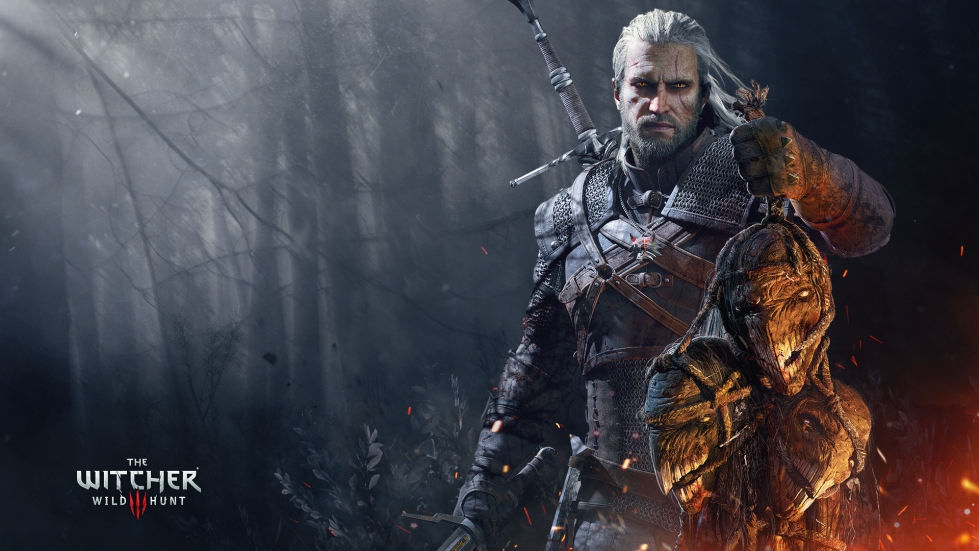
\includegraphics[width=1\textwidth]{witcher}
  \caption{3D Graphics}
  \end{figure}
  %\vspace{3cm} 
  \end{column}
  \begin{column}{6cm}
  \begin{figure}
  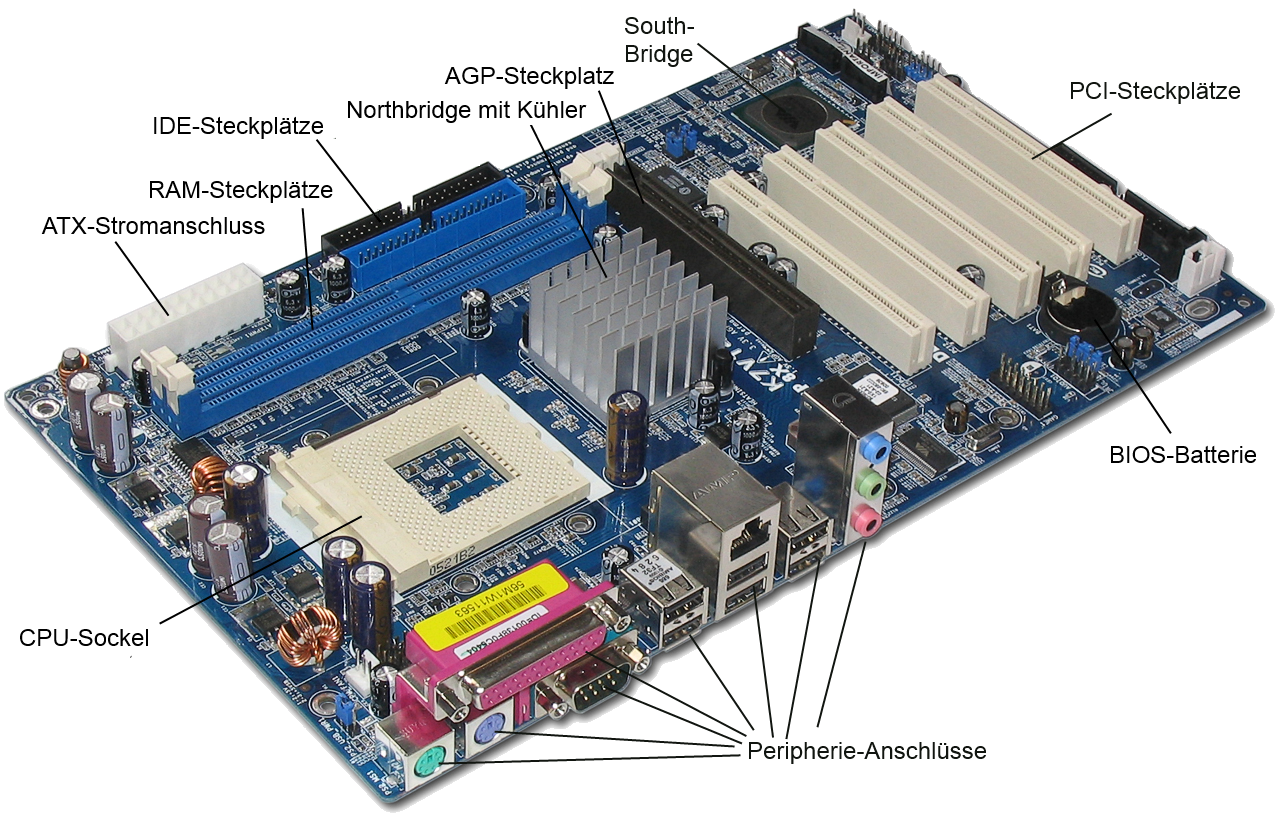
\includegraphics[width=1\textwidth]{motherboard}
  \caption{Motherboard}
  \end{figure}
  \end{column}
  \end{columns}
\end{frame}


\begin{frame}\frametitle{What do we need?}
  \begin{columns}
  \begin{column}{6cm}
  \begin{figure}
  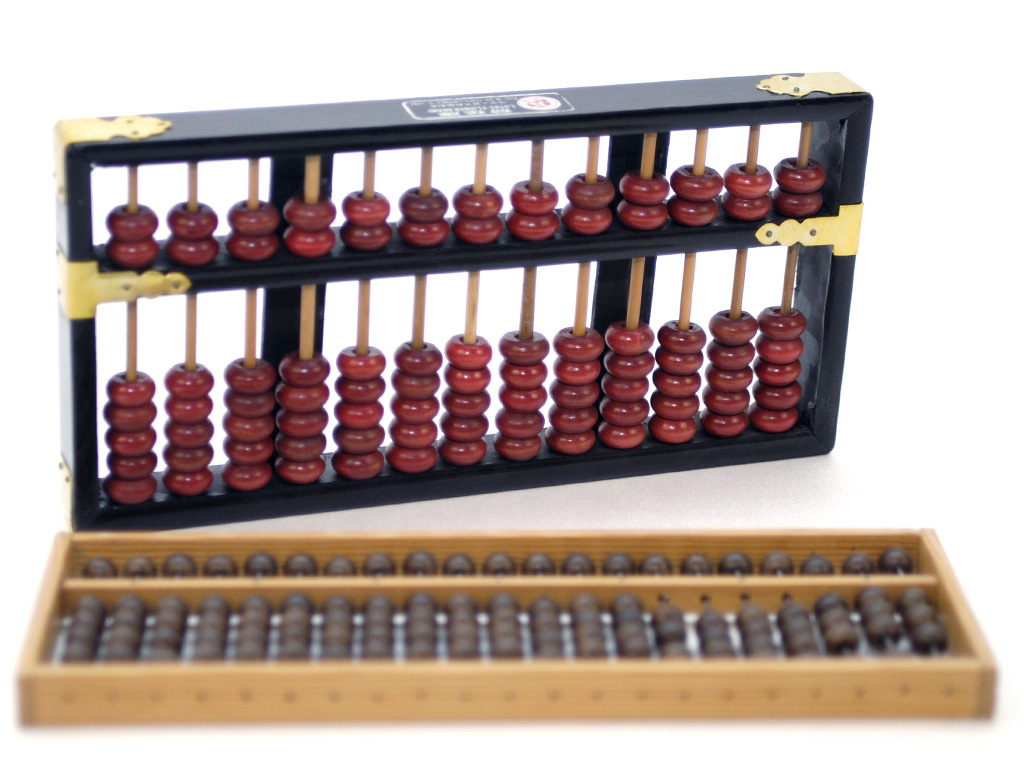
\includegraphics[width=1\textwidth]{abakus}
  \caption{Abakus}
  \end{figure}
  %\vspace{3cm} 
  \end{column}
  \begin{column}{6cm}
  \begin{figure}
  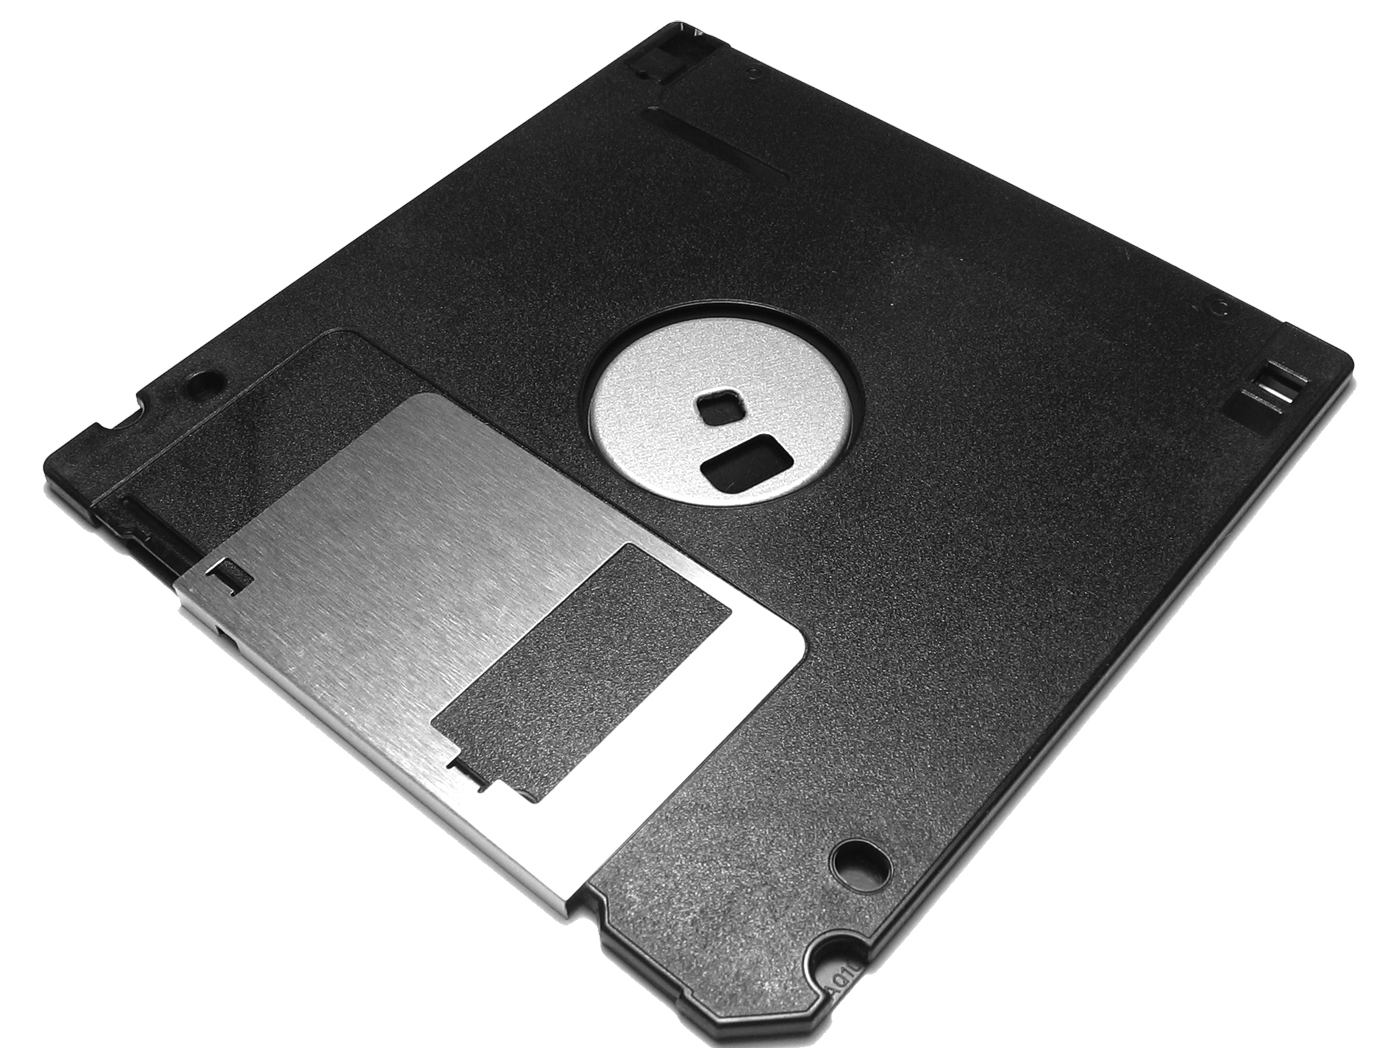
\includegraphics[width=1\textwidth]{memory}
  \caption{Memory}
  \end{figure}
  \end{column}
  \end{columns}
\end{frame}







\end{document}